\chapter{Quick\_Plot Plotting}
\label{c:quick_plot}
\index{Quick_Plot|textbf}
\index{PGPLOT!and Quick_Plot}

The plotting package included in the \bmad distribution is PGPLOT
(see \sref{s:libs}).
One drawback of PGPLOT is that the arguments to
PGPLOT's subroutines are not always conveniently structured. to remedy
this a suite of wrapper routines have been developed which can be
used to drive PGPLOT. This suite is called \quickplot and lives in the
\vn{dcslib} library which comes with the Bmad distribution. A quick
reference guide can be seen online by using the command \vn{getf
quick_plot}. For quick identification in a program, all \quickplot
subroutines start with a \vn{qp_} prefix. Also, by convention, all
PGPLOT subroutines start with a \vn{pg} prefix.

While \quickplot covers most of the features of PGPLOT, \quickplot is
still a work in progress.  For example, contour plots have not yet
been implemented in \quickplot. If you see a feature that is lacking
in \quickplot please do not hesitate to make a request to
\vn{dcs16@cornell.edu}.

Note: PGPLOT uses single precision real(4) numbers while \quickplot
uses real(rp) numbers.  If you use any PGPLOT subroutines directly be
careful of this.

%----------------------------------------------------------------------------

\begin{figure}
\footnotesize
\begin{listing}{1}
  program example_plot
    use quick_plot
    integer id
    character(1) ans
  
  ! Generate PS and X-windows plots.
    call qp_open_page ("PS-L")  ! Tell \quickplot to generate a PS file.
    call plot_it              ! Generate the plot
    call qp_close_page        ! quick_plot.ps is the file name
    call qp_open_page ("X", id, 600.0_rp, 470.0_rp, "POINTS")
    call plot_it
    write (*, "(a)", advance = "NO") " Hit any key to end program: "
    accept "(a)", ans

  !----------------------------------------------------------------------
  contains
  subroutine plot_it                             ! This generates the plot
    real(rp), allocatable :: x(:), y(:), z(:), t(:)
    real(rp) x_axis_min, x_axis_max, y_axis_min, y_axis_max
    integer x_places, x_divisions, y_places, y_divisions
    character(80) title
    logical err_flag
    namelist / parameters / title

  ! Read in the data
    open (1, file = "plot.dat", status = "old")
    read (1, nml = parameters)                  ! read in the parameters.
    call qp_read_data (1, err_flag, x, 1, y, 3, z, 4, t, 5) ! read in the data.
    close (1)

  ! Setup the margins and page border and draw the title
    call qp_set_page_border (0.01_rp, 0.02_rp, 0.2_rp, 0.2_rp, "%PAGE")
    call qp_set_margin (0.07_rp, 0.05_rp, 0.05_rp, 0.05_rp, "%PAGE")
    call qp_draw_text (title, 0.5_rp, 0.85_rp, "%PAGE", "CT") 

  ! draw the left graph
    call qp_set_box (1, 1, 2, 1)
    call qp_calc_and_set_axis ("X", minval(x), maxval(x), 4, 8, "ZERO_AT_END")
    call qp_calc_and_set_axis ("Y", minval(z), maxval(z), 4, 8, "GENERAL")
    call qp_draw_graph (x, y, "X\dlab\u", "\gb(\A)", symbol_every = 0)

    call qp_save_state (.true.)
    call qp_set_symbol_attrib (times$, color = blue$, height = 20.0_rp)
    call qp_set_line_attrib ("PLOT", color = blue$, style = dashed$)
    call qp_draw_data (x, z, symbol_every = 5)
    call qp_restore_state

  ! draw the right graph. star5_filled$ is a five pointed star.
    call qp_save_state (.true.)
    call qp_set_box (2, 1, 2, 1)
    call qp_set_graph_attrib (draw_grid = .false.)
    call qp_set_symbol_attrib (star5_filled$, height = 10.0_rp)
    call qp_set_axis ("Y", -0.1_rp, 0.1_rp, 4, 2)
    call qp_set_axis ("Y2", label = "Y2 axis")
    call qp_draw_graph (x, t, "\m1 \m2 \m3 \m4 \m5 \m6 \m7", "\fsLY\fn", &
             title = "That Darn Graph", draw_line = .false., symbol_every = 4)
    call qp_restore_state
  end subroutine
  end program
\end{listing}
\caption{\quickplot example program.}
\label{f:plot_example}
\end{figure}


\begin{figure}
\centering
\includegraphics[width=5.5in]{plot_example.psfig}
\caption{Output of plot\_example.f90.}
\label{f:plot_out}
\end{figure}

%----------------------------------------------------------------------------
\section{An Example}
\label{s:plot_example}

An example of how \quickplot can be used in a program is shown in
Figure~\ref{f:plot_example}. In the \bmad distribution a copy of this
program is in the file
\begin{example}
  dcslib/plot_example.f90
\end{example}
The \vn{plot_example.f90} program generates the figure shown in
Figure~\ref{f:plot_out} from the input file named \vn{plot.dat}. The
first few lines of the data file are
\begin{example}
  \&parameters
    title = "A Tale of Two Graphs"
  /
 
  Any junk here...
 
  Col1      Col2      Col3      Col4      Col5
     0    0.0000    0.1000    0.0000   -0.0125
     1    0.0001    0.0995    0.0101   -0.0127
     2    0.0004    0.0980    0.0203   -0.0130
     3    0.0009    0.0955    0.0304   -0.0132
     ...
\end{example}

The program first creates a PostScript file for printing on lines 7
through 9 and then makes an X--windows plot on lines 10 and 11. The
write/accept lines 12 and 13 are to pause the program to prevent the
X-window from immediately closing upon termination of the program.

The heart of the plotting is in the subroutine \vn{plot_it} beginning
on line 18. The namelist read on line 28 shows how both parameters and
data can be stored in the same file so that a plotting program can be
automatically told what the appropriate plot labels are. The
\vn{qp_draw_text} call on line 35 draws the title above the two graphs.

The \vn{qp_read_data} routine on line 29 will skip any ``header''
lines (lines that do not begin with something that looks like a
number). In this instance \vn{qp_read_data} will read the first, third
forth and fifth data columns and put them into the \vn{x}, \vn{y},
\vn{z}, and \vn{t} arrays.

\vn{qp_set_page_border}, \vn{qp_set_box}, and \vn{qp_set_margin} sets
where the graph is going to be placed (see below for more details).
\vn{qp_set_box(1, 1, 2, 1)} on line 38 tells \quickplot to put the
first graph in the left box of a 2 box grid. The \vn{qp_set_margin} on
line 34 sets the margins between the box and the graph axes.

\vn{qp_calc_and_set_axis} on lines 39 and 40 are used to scale the
axes. \vn{"ZERO_AT_END"} ensures that the $x$--axis starts (or stops)
at zero.  \vn{qp_calc_and_axis_axis} is told to restrict the number of
major divisions to be between 4 and 8. For the horizontal axis, as can be
seen in Figure~\ref{f:plot_out}, it chooses 5 divisions.

After drawing the first data curve (the solid curve) in the left
graph, the routines \vn{qp_set_symbol_attrib} and
\vn{qp_set_line_attrib} are called on lines 44 and 45 to plot the next
data curve in blue with a dashed line style. By default this curve
goes where the last one did: in the left graph. To keep the setting of
the line and symbol attributes from affecting other plots the routines
\vn{qp_save_state} and \vn{qp_restore_state} on lines 43 and 47 are
used. \vn{qp_save_state} saves the current attributes in a attribute
stack. \vn{qp_restore_state} restores the saved attributes from the
attribute stack. \vn{qp_draw_data} on line 46 is similar to
\vn{qp_draw_graph} except only the data is drawn. Not the axes and
associated labels.

Lines 50 through 57 draw the third curve in the right hand graph.
Line 55 labels the \vn{y2} (right hand) axis. The syntax of the
string arguments of \vn{qp_draw_graph} in lines 41 and 56/57 comes
from PGPLOT and allows special symbols along with subscripts and
superscripts.

%----------------------------------------------------------------------------
\section{Plotting Coordinates}
\label{s:plot_coords}

\begin{figure}
  \centering
  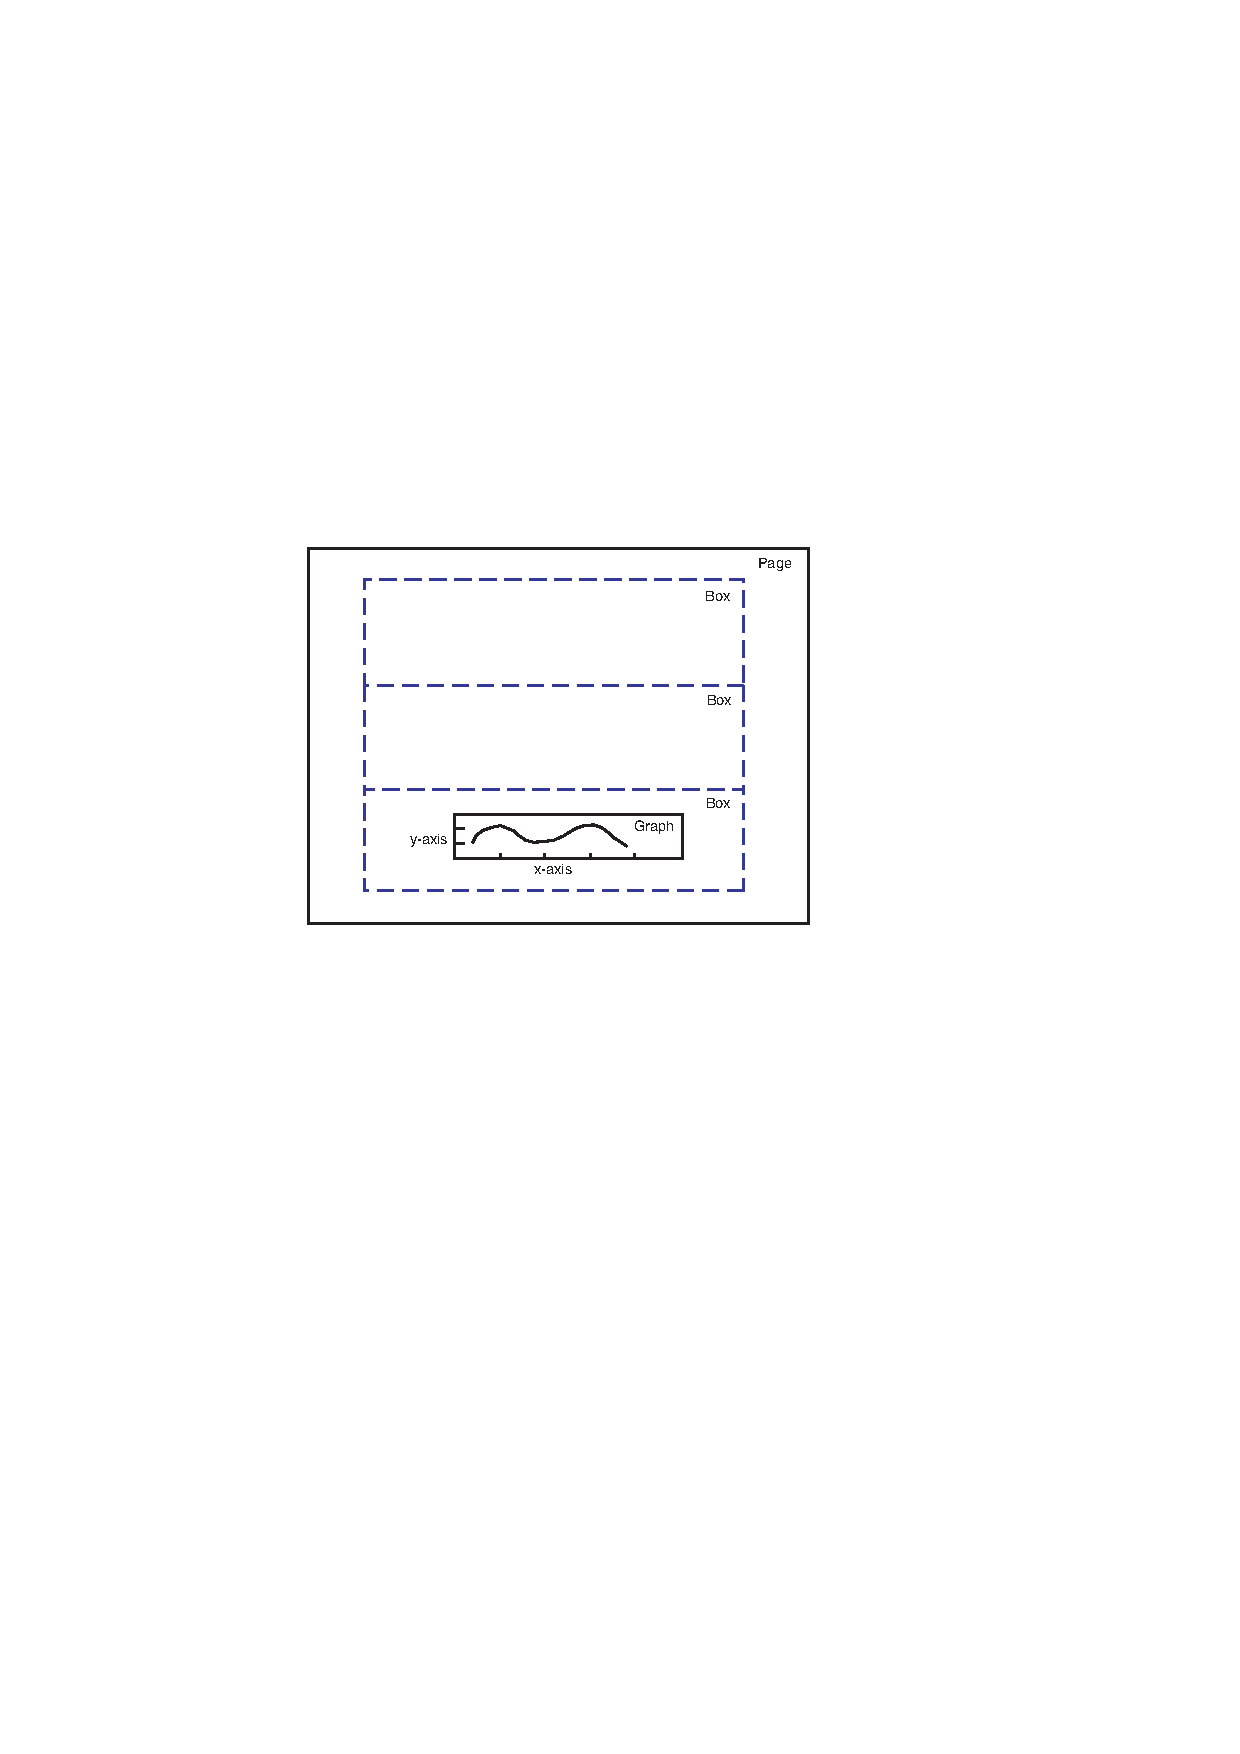
\includegraphics{plot_coords.psfig}
  \caption{A Graph within a Box within a Page.}
  \label{f:plot_coords}
\end{figure}

\quickplot uses the following concepts as shown in Figure~\ref{f:plot_coords}
\begin{example}
  PAGE  -- The entire drawing surface.
  BOX   -- The area of the page that a graph is placed into.
  GRAPH -- The actual plotting area within the bounds of the axes.
\end{example}
In case you need to refer to the PGPLOT routines the correspondence between this and PGPLOT is:
\begin{example}
  QUICK_PLOT    PGPLOT
  ----------    ------
  PAGE          VIEW SURFACE
  BOX           No corresponding entity.
  GRAPH         VIEWPORT and WINDOW
\end{example}
Essentially the VIEWPORT is the region outside of which lines and symbols
will be clipped (if clipping is turned on) and the WINDOW defines the
plot area. I'm not sure why PGPLOT makes a distinction but VIEWPORT and
WINDOW always are the same region.

\vn{qp_open_page} determines the size of the \vn{page} if it is settable (like for
X--windows). The page is divided up into a grid of boxes. For example, 
in Figure~\ref{f:plot_coords}, the grid is 1 box wide by 3 boxes tall. The border
between the grid of boxes and the edges of the page are set by \vn{qp_set_page_border}.
The box that the graph falls into is set by \vn{qp_set_box}. The default is to
have no margins with 1 box covering the entire page. The \vn{qp_set_margin} routine
sets the distance between the box edges and the axes.


%----------------------------------------------------------------------------
\section{Length and Position Units}
\label{s:plot_units}
\index{Quick_Plot!position units}

Typically there is an optional \vn{units} argument for \quickplot routines that
have length and/or position arguments. For example, using \vn{getf} one can
see that the arguments for \vn{qp_draw_rectangle} are
\begin{example}
  Subroutine qp_draw_rectangle (x1, x2, y1, y2, units, color, width, style, clip)
\end{example}
The \vn{units} argument is a character string which is divided into three
parts. The syntax of the \vn{units} argument is
\begin{example}
  unit_type/ref_object/corner
\end{example}
The first part \vn{unit_type} gives the type of units
\begin{example}
  "%"       -- Percent.
  "DATA"    -- Data units. (Draw default)
  "MM"      -- millimeters.
  "INCH"    -- Inches. (Set default)
  "POINTS"  -- Printers points (72 points = 1 inch, 1pt is about 1pixel).
\end{example}
The second and third parts give the reference point for a position.
The second part specifies the reference object
\begin{example}
    "PAGE"  -- Relative to the page (Set default).
    "BOX"   -- Relative to the box.
    "GRAPH" -- Relative to the graph (Draw default).
\end{example}
The third part gives corner of the reference object that is the reference point
\begin{example}
    "LB"    -- Left Bottom (Set and Draw default).
    "LT"    -- Left Top.
    "RB"    -- Right Bottom.
    "RT"    -- Right Top.
\end{example}

Notes:
\begin{itemize}
 \item 
The \vn{DATA} unit type, by definition, always uses the lower left
corner of the \vn{GRAPH} as a reference point.
 \item 
For the \vn{%} \vn{unit_type} the \vn{/} between \vn{unit_type} 
and \vn{ref_object} can be omitted.
 \item 
If the \vn{corner} is specified then the \vn{ref_object} must appear also.
 \item 
Everything must be in upper case.
 \item 
For some routines (\vn{qp_set_margin}, etc.) only a relative distance
is needed. In this case the \vn{ref_object/corner} part, if present,
is ignored.
 \item 
The \vn{units} argument is typically an optional argument. If not
present the default units will be used. There are actually two
defaults: The draw default is used for drawing text, symbols, or whatever.
The set default is used for setting margins, and other lengths.
Initially the draw default is \vn{DATA/GRAPH/LB} and the set
default is \vn{INCH/PAGE/LB}. use \vn{qp_set_default} to change this.
\end{itemize}
Examples:
\begin{example}
  "DATA"          -- This is the draw default. 
  "DATA/GRAPH/LB" -- Same as above.
  "DATA/BOX/RT"   -- ILLEGAL: DATA must always go with GRAPH/LB.
  "%PAGE/LT"      -- Percentage of page so (0.0, 1.0) = RT of page.
  "%BOX"          -- Percentage of box so (1.0, 1.0) = RT of box.
  "INCH/PAGE"     -- Inches from LB of page.
\end{example}

%----------------------------------------------------------------------------
\section{Y2 and X2 axes}
\label{s:axes2}
\index{Quick_Plot!axes}

The top and right axes of a graph are known as \vn{X2} and \vn{Y2}
respectively as shown in Figure~\ref{f:plot_coords}. Normally the
\vn{X2} axis mirrors the \vn{X} axis and the \vn{Y2} axis mirrors the
\vn{Y} axis in that the tick marks and axis numbering for the \vn{X2}
and \vn{Y2} axes are the same as the \vn{X} and \vn{Y} axes
respectively. \vn{qp_set_axis} can be used to disable mirroring. For example:
\begin{example}
  call qp_set_axis ("Y2", mirror = .false.)  ! y2-axis now independent of y.
\end{example}
\vn{qp_set_axis} can also be used to set \vn{Y2} axis parameters (axis
minimum, maximum, etc.). 

Note that the default is for the \vn{X2} and \vn{Y2} axis numbering
not to be shown. To enable or disable axis numbering again use
\vn{qp_set_axis}. For example:
\begin{example}
  call qp_set_axis ("Y2", draw_numbers = .true.)  ! draw y2 axis numbers
\end{example}

%----------------------------------------------------------------------------
\section{Styles}
\label{s:styles}

Symbolic constants have been defined for \quickplot subroutine
arguments that are used to choose various styles. As an example of
this is in lines 44 and 45 of Figure~\ref{f:plot_example}. The
numbers in the following are the PGPLOT equivalents.

\index{Quick_Plot!line styles}
The \quickplot line styles are:
\begin{example}
    1 -- solid\$                  Solid
    2 -- dashed\$                 Dashed
    3 -- dash_dot\$               Dash--dot 
    4 -- dotted\$                 Dotted
    5 -- dash_dot3\$              Dash--dot--dot--dot        
\end{example}

\index{Quick_Plot!color styles}
The color styles in \quickplot are:
\begin{example}
    0 -- White\$   (actually the background color)
    1 -- Black\$   (actually the foreground color)
    2 -- Red\$
    3 -- Green\$
    4 -- Blue\$
    5 -- Cyan\$
    6 -- Magenta\$
    7 -- Yellow\$ 
    8 -- Orange\$
    9 -- Yellow_Green\$
   10 -- Light_Green\$
   11 -- Navy_Blue\$
   12 -- Purple\$
   13 -- Redish_Purple\$
   14 -- Dark_Grey\$
   15 -- Light_Grey\$
\end{example}

\index{Quick_Plot!fill styles}
The fill styles are:
\begin{example}
    1 -- solid_fill\$        
    2 -- no_fill\$           
    3 -- hatched\$           
    4 -- cross_hatched\$     
\end{example}

\index{Quick_Plot!symbol table}
\begin{table}
  \centering
  \includegraphics{plot_syms.psfig}
  \caption{Plotting Symbols at Height = 40.0}
  \label{t:plot_syms}
\end{table}

\index{Quick_Plot!symbol styles}
The symbol types are:
\begin{example}
    0 -- square\$
    1 -- dot\$
    2 -- plus\$
    3 -- times\$
    4 -- circle\$
    5 -- x_symbol\$
    7 -- triangle\$
    8 -- circle_plus\$
    9 -- circle_dot\$
   10 -- square_concave\$
   11 -- diamond\$
   12 -- star5\$
   13 -- triangle_filled\$
   14 -- red_cross\$
   15 -- star_of_david\$
   16 -- square_filled\$
   17 -- circle_filled\$
   18 -- star5_filled\$
\end{example}
Beside this list, PGPLOT maps other numbers onto symbol types. 
The PGPLOT list of symbols is:
\begin{example}
  -3 ... -31 - a regular polygon with abs(type) edges.
          -2 - Same as -1.
          -1 - Dot with diameter = current line width.
   0 ...  31 - Standard marker symbols.
  32 ... 127 - ASCII characters (in the current font).
                  E.G. to use letter F as a marker, set type = ICHAR("F"). 
       > 127 - A Hershey symbol number.
\end{example}
Table~\ref{t:plot_syms} shows some of the symbols and there associated 
numbers. Note: At constant height PGPLOT gives symbols of different size.
To partially overcome this, \quickplot scales some of the symbols to
give a more uniform appearence. Table~\ref{t:plot_syms} was generated
using a height of 40 via the call
\begin{example}
  call qp_draw_symbol (0.5_rp, 0.5_rp, "%BOX", k, height = 40.0_rp)
\end{example}

PGPLOT defines certain escape sequences that can be used in text strings
to draw greek letters, etc. These escape sequences are given in 
Table~\ref{t:pgplot_escape}.
\begin{table}[h]
\begin{tabular}{|l|l|} \hline
{\B}u       & Start a superscript, or end a subscript \\ \hline
{\B}d       & \parbox{4in}{Start a subscript, or end a superscript 
               (note that {\B}u and {\B}d must always be used in pairs)} \\ \hline
{\B}b       & \parbox{4in}{Backspace (i.e., do not advance text pointer  
               after plotting the previous character)} \\ \hline
{\B}fn      & Switch to Normal font (1)       \\ \hline
{\B}fr      & Switch to Roman font (2)        \\ \hline
{\B}fi      & Switch to Italic font (3)       \\ \hline
{\B}fs      & Switch to Script font (4)       \\ \hline
{\B}{\B}    & Backslash character (\B)        \\ \hline
{\B}x       & Multiplication sign ($\times$)  \\ \hline
{\B}.       & Centered dot ($\cdot$)          \\ \hline
{\B}A       & Angstrom symbol (\AA)         \\ \hline
{\B}gx      & Greek letter corresponding to roman letter x \\ \hline
{\B}mn {\B}mnn & Graph marker number $n$ or $nn$ (1-31) \\ \hline
{\B}(nnnn)  & 
\parbox{4in}{Character number nnnn (1 to 4 decimal digits) from the
Hershey character set; the closing parenthesis may be omitted if the
next character is neither a digit nor ``)''. This makes a number of
special characters (e.g., mathematical, musical, astronomical, and
cartographical symbols) available.} \\ \hline
\end{tabular}
\caption{PGPLOT Escape Sequences.}
\label{t:pgplot_escape}
\end{table}

PGPLOT defines a text background index:
\begin{example}
         -1 - Transparent background.
          0 - Erase underlying graphics before drawing text.
   1 to 255 - Opaque with the number specifying the color index.
\end{example}

%----------------------------------------------------------------------------
\section{Structures}
\label{s:qp_structs}
\index{Quick_Plot!structures}

\quickplot uses several structures to hold data. The structure that
defines a line is called a \vn{qp_line_struct} and is shown in
Figure~\ref{f:qp_line_struct}. 
\begin{figure}[htb]
\centering
\begin{verbatim}
  type qp_line_struct
    integer width   ! Line width. Default = 1
    integer color   ! Line color. Default = black\$
    integer style   ! Line style. Default = solid\$
  end type
\end{verbatim}
\caption{Definition of the \vn{qp\_line\_struct}.}
\label{f:qp_line_struct}
\end{figure}

The \vn{qp_symbol_struct} defines how symbols are drawn and is shown
in Figure~\ref{f:qp_sym_struct}.
\begin{figure}[htb]
\centering
\begin{verbatim}
  type qp_symbol_struct
    integer  type        ! Default = circle_dot\$
    real(rp) height      ! Default = 6.0 (points)
    integer  color       ! Default = black\$
    integer  fill        ! Default = solid_fill\$
    integer  line_width  ! Default = 1
  end type
\end{verbatim}
\caption{Definition of the \vn{qp\_sym\_struct}.}
\label{f:qp_sym_struct}
\end{figure}

The \vn{qp_axis_struct} defines how axes are drawn and is shown
in Figure~\ref{f:qp_axis_struct}.
\begin{figure}[htb]
\centering
\begin{verbatim}
  type qp_axis_struct
    character(80) label       ! Axis label.
    real(rp) min              ! Axis minimum number.
    real(rp) max              ! Axis maximum number.
    real(rp) number_offset    ! Offset of numbering from the axis line.
    real(rp) label_offset     ! Offset of the label from the numbering.
    real(rp) major_tick_len   ! Length of the major ticks in inches.
    real(rp) minor_tick_len   ! Length of the minor ticks in inches.
    integer major_div         ! Number of major divisions.
    integer minor_div         ! Number of minor divisions.
    integer minor_div_max     ! Maximum number for auto choose.
    integer places            ! Places after the decimal point.
    character(16) type        ! For log scales. Not yet implemented.
    integer tick_side         ! +1 = draw to the inside, 0 = both, -1 = outside.
    integer number_side       ! +1 = draw to the inside, -1 = outside.
    logical draw_label        ! Draw the label?
    logical draw_numbers      ! Draw the numbering?
  end type
\end{verbatim}
\caption{Definition of the \vn{qp\_axis\_struct}.}
\label{f:qp_axis_struct}
\end{figure}


